\chapter{Bevezetés}
\label{ch:intro}

A modern szoftverfejlesztés egyik népszerű tautológiája, hogy minőségi, hosszú távon is karbantartható szoftvert fejleszteni nehéz. Ennek sok különböző oka, de a probléma központja az, hogy egyszerűen nehéz definiálni, hogy a "jó" és a "minőségi" szavak pontosan mit is jelentenek egy kódbázis esetében. Hiába áll közel a matematika egzakt természetéhez egy kontextus nélkül értelmezett kódsor, minél nagyobb halmazát nézzük távolról egy kódsor halmaznak, annál közelebb kerülünk a filozófiából ismerős minőség erősen homályos koncepciójához.

A tapasztalatra hivatkozhatnánk a minőség egyik prediktoraként, hiszen ha valami bevált korábban több projekten, akkor egy n+1-edik projekten is működni fog. Ez a feltételezés természetesen nem állja meg a helyét. Amellett, hogy a status quo folyamatos megkérdőjelezése előbb fog jó minőségű szoftverhez vezetni, mint annak a vak követése, azt is fontos megjegyezni, hogy egy szoftver projekt kontextusának csak egyik vektora a konkrét kód és a mögötte lévő követelmény. A fejlesztő csapat, a csapat és a csapatot alkalmazó cég kultúrája jelentősen torzítják a korábbi tapasztalat alkalmazásának hasznosságát. Melvin Conway programozó 1967-ben tett egy azóta elhíresült kijelentést, amelyre évtizedek óta csak Conway törvényeként\cite{conway} hivatkozunk:
\begin{quotation}
    Any organization that designs a system (defined broadly) will produce a design whose structure is a copy of the organization's communication structure.
\end{quotation}

Conway törvénye azt fogalmazza meg, hogy egy szervezet szoftverei jellemzően tükrözni fogják a szervezet kommunikációs struktúráját. Ez hatással van a korábban említett tapasztalati faktorra: egy szervezetben fejlesztett szoftver és a hozzá tartozó gyakorlatok nem feltétlenül illeszkednek egy másik szervezetben fejlesztett szoftver követelményeire.

Friss vezető fejlesztőként, 2019-ben futottam bele a következő kérdésbe: milyen objektív, empirikus statisztikát alkalmazhatnék egy fejlődő kódbázis elemzésére, ami mentes a saját minőségi kóddal kialakított koncepcióimtól? Ekkor futottam bele az azt megelőző évben megjelent, \textit{Software Design X-Rays}\cite{tornhillXrays} című könyvbe, ami egy számomra új, gyakorlatban hasznosítható megközelítést prezentál a kódbázisokat gyakori problémáinak felismerésére, programozási nyelvtől, paradigmától és platformtól függetlenül.

Az ötlet egyszerű: minden olyan szoftverfejlesztési projekt, ahol a minőség akármilyen szinten releváns, ott a kód verziókezelő rendszerben van tárolva. Ezek a verziókezelő rendszerek nagyon specifikus célokat szolgálnak (erről bővebben az \ref{section:version_control} szekcióban), azonban rengeteg metaadatot tárolnak a kódról projekt, fájl és sor szintjén is.

\citeauthor{tornhillXrays} két statisztikai pontra hivatkozik a könyvében:
\begin{enumerate}
    \item Egy fájl, vagy fájlban lévő sor hányszor került módosításra
    \item Egy fájl, vagy fájlban lévő sor hány különböző szerző által lett módosítva
\end{enumerate}

A feltételezés, hogy a kódbázisok problémás részein kiemelkedően magas lesz a fent említett két szám az kódbázis többi részéhez képest. Továbbá feltehető az is, hogy azok a fájlok, amiken ez megfigyelhető, azok a fejlesztés korai szakaszaitól jelen vannak és a módosítások száma a projekt életciklusa alatt nagyjából konstans marad.

Jogos kérdés lehet, hogy pontosan miért probléma az, hogy egy fájlt, illetve a benne lévő osztályt gyakran kell módosítani. Ehhez egy pillanatra hátra kell lépnünk és szót kell ejtenünk az úgynevezett code smell-ekről.

\section{Code smell}

A code smell, mint koncepció Martin Fowler \textit{Refactoring}\cite{fowlerRefactoring} című könyvével került be a programozói köztudatba. \textit{Code smell} alatt jellemzően olyan kódot értünk, aminek a működése szigorúan vett értelemben nem helytelen, azonban szoftver dizájn szempontból egészségtelen a kód hosszú távú karbantarthatóságára nézve.

Fowler a könyvében 16 különböző code smell-t definiál, amiből nekünk a következőek relevánsak:
\begin{enumerate}
    \item \textit{Long method}: szükségtelenül hosszú függvény, ami indokolatlanul sok operációt végez, nem fókuszált
    \item \textit{Large class}: indokolatlanul nagy osztály, ami reálisan több különálló osztály logikáját tartalmazza. Gyakorlatban \textit{God Class} vagy \textit{God Object} néven hivatkozunk erre a code smell-re
    \item \textit{Divergent change}: egy változtatás végrehajtásához sok, egymástól független függvény megváltoztatása szükséges
    \item \textit{Shotgun surgery}: egy kis változtatás sikeres végrehajtása csak sok osztály megváltoztatásával lehetséges
\end{enumerate}

Fontos megjegyezni, hogy a code smell, mint olyan, pusztán egy felületi heurisztika: egy kódrészlet, amire egy, vagy akár több code smell is illeszkedik, az a saját kontextusában lehet dizájn szempontból is helyes, hiszen minden szoftver projekt más. Az code smell-ek értéke abban rejlik, hogy a segítségükkel gyorsan fel tudunk ismerni gyakran előforduló problémás mintákat, majd egyéni mérlegelés után dönthetünk arról, hogy szükséges-e változtatást eszközölni a gyanús kódon.

\section{Verziókezelő}
\label{section:version_control}

A verziókezelő szerves részeit képzik a modern szoftverfejlesztésnek. A fejlesztői körökben híres \textit{Joel Test}\footnote{https://www.joelonsoftware.com/2000/08/09/the-joel-test-12-steps-to-better-code/} legelső lakmusz-tesztje, hogy egy projekt minden forráskódjának valamilyen formában verziókezelőben kell lennie, máskülönben (Spolsky véleménye szerint) a fejlesztők csak a saját és a klienseik életét nehezítik meg.

De mi is pontosan egy verziókezelő? Egy verziókezelő szoftver célja, hogy a forráskódon történő változtatások mindig világosan visszakövethetőek legyenek, egyértelműen látszódjon a változtatás előtti és utáni állapot és a forráskód akármelyik állapota akármikor elérhető és visszaállítható legyen. Fontos továbbá az is, hogy a verziókezelő rendszerek úgynevezett branch-ek használatával elősegítik, hogy egy fejlesztő csapat minden tagja képes legyen ugyanazokon a fájlokon más-más változtatásokat végrehajtani úgy, hogy a potenciálisan létrejött konfliktusokat csak egyszer kell feloldani.

Koncepcionálisan a verziókezelőket, illetve az azokban tárolt forráskódot nagyon komplex gráfként érdemes elképzelni, ahol minden csúcs a forráskód egy bizonyos állapota.

A legismertebb verziókezelők:
\begin{itemize}
    \item \textit{SVN}: a 2000-es évek elejének legnépszerűbb, centralizált verziókezelő rendszere.
    \item \textit{Perforce}: centralizált verziókezelő, ami koncepcionálisan az SVN-hez közelít, azonban nem nyílt forráskódú. Nagy céges környezetben a mai napig viszonylag népszerű, köszönhetően főleg annak, hogy kiválóan képes kezelni a bináris fájlokat.
    \item \textit{git}: messze a legnépszerűbb modern, decentralizált verziókezelő rendszer. Bővebben részletezve a következő szekcióban.
\end{itemize}

Terminológia szempontjából a következők lesznek fontosak:
\begin{itemize}
    \item \textit{Repository}: egy megosztott adatbázis, ami tartalmazza a verziókezelt forráskód összes különböző verziójának állapotát
    \item \textit{Commit}: változtatások egy halmaza, ami a forráskód egy korábbi változatát egy új verzióra képezi le
    \item \textit{Branch}: a forráskód egy bizonyos commit-járól való leágazás, ami egy, a szülő branch-től független commit történettel fog rendelkezni a vágási ponttól
\end{itemize}

\subsection{A legnépszerűbb verziókezelő - git}

Az elmúlt évtizedben a git messze kiemelkedett

\begin{figure}[H]
    \centering
    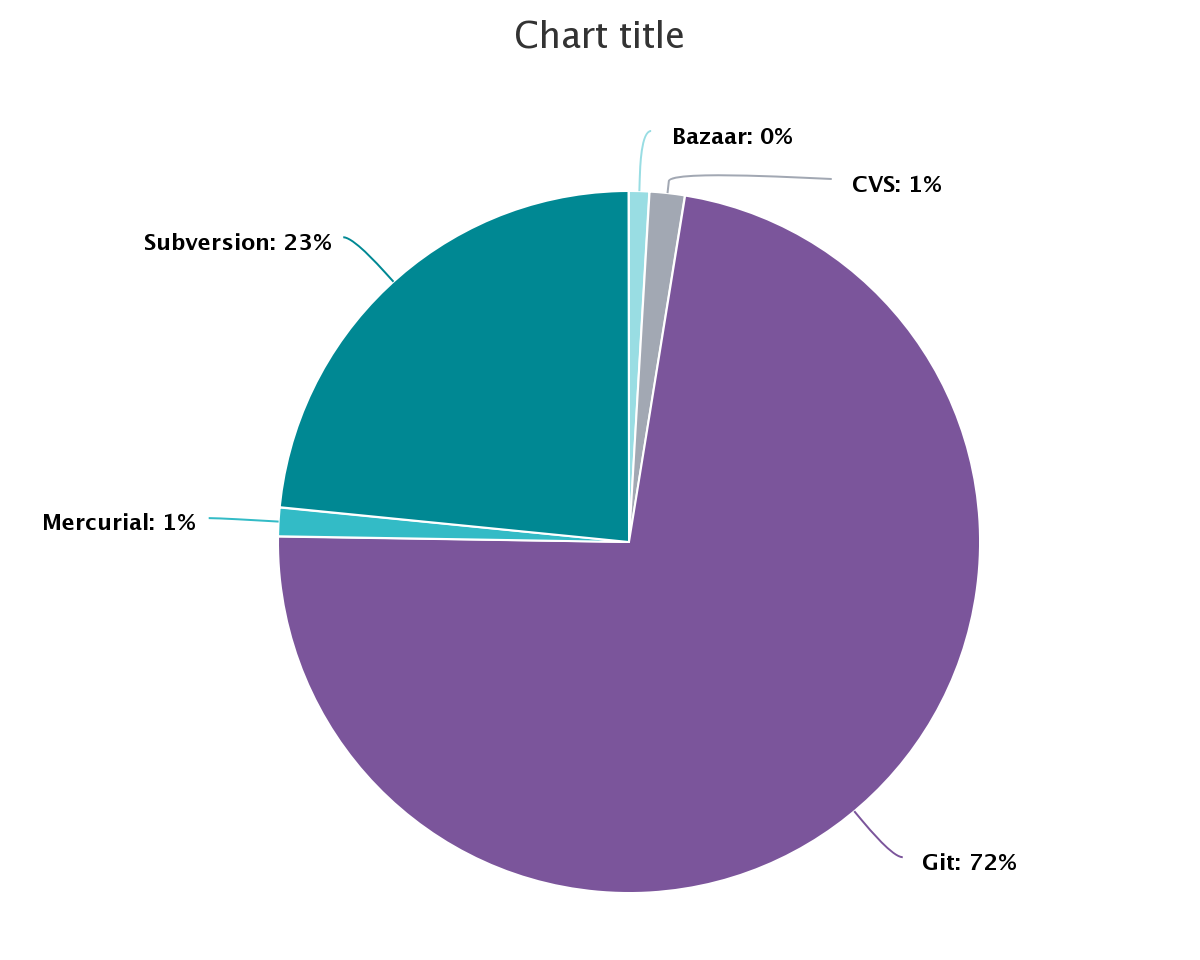
\includegraphics[width=0.8\textwidth]{images/gitMarketShare.png}
    \caption{Verziókezelők relatív népszerűsége 2020-ban}
    \label{fig:version-controls}
\end{figure}

\begin{figure}[H]
    \centering
    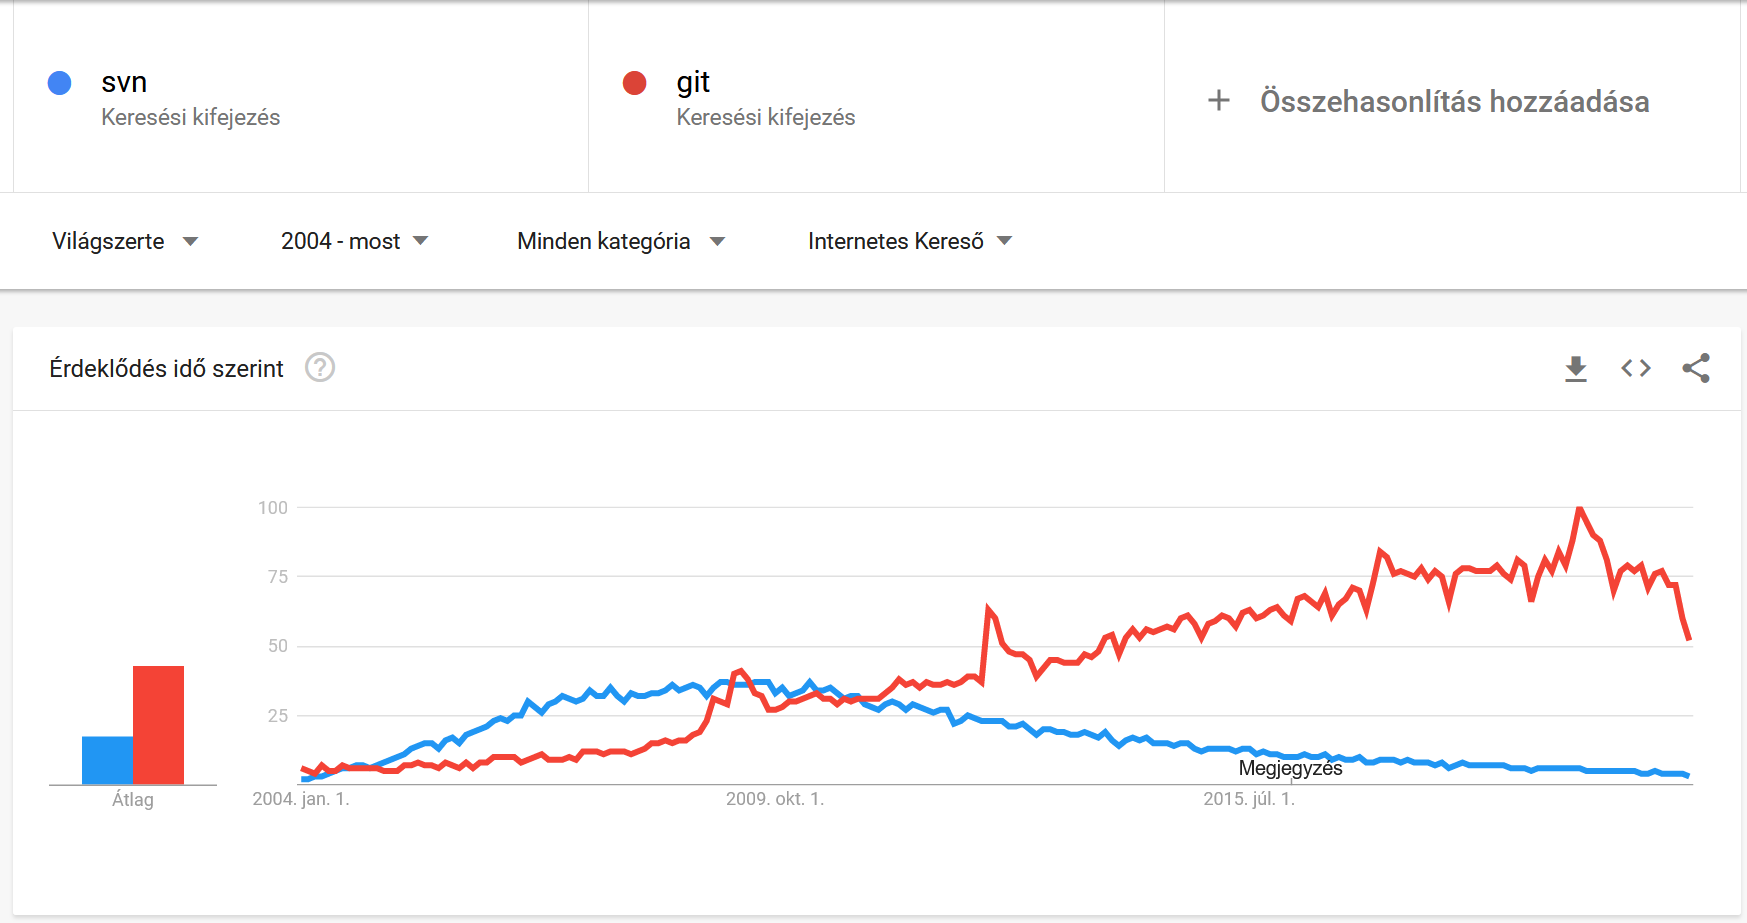
\includegraphics[width=0.8\textwidth]{images/gitsvn.png}
    \caption{A git és SVN népszerűségének változása Google Trends szerint 2004 és 2020 között}
    \label{fig:git-svn-trends}
\end{figure}


Hála az open source közösség által felkarolt GitHub-nak, az elmúlt évtizedben a git lett az ipar de facto verziókezelője. A korábban említett alternatívákkal szemben a git teljesen decentralizált, ami azt jelenti, hogy nincs egy központi igazságként szolgáló repository, hanem egy git repository minden másolata teljes értékű. Természetesen mivel másolatokról beszélünk, ez implikálja, hogy mégis van egy

\subsection{Code smell-ek nyomai a verziókezelőben}

Itt az ideje részleteiben kitérni a \textit{Software Design X-Rays}\cite{tornhillXrays} kapcsán már említett git statisztikákra, illetve a

Egy modern kutatás, ami kifejezetten a code smell-ek empirikus felismerésével foglakozik 2015-ben került publikálásra M. Tufano et al., "When and Why Your Code Starts to Smell Bad"\cite{codeSmells}.

\section{Tesztelés}

A modern szoftverfejlesztés egyik legnagyobb előrelépése

\begin{figure}[H]
    \centering
    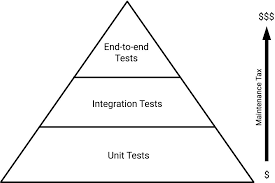
\includegraphics[width=0.8\textwidth]{images/piramis.png}
    \caption{Tesztelési piramis}
    \label{fig:testing-pyramid}
\end{figure}

\subsection{Magasabb szintű tesztek}

A tesztelési piramis legfelsőbb szintjén találjuk az E2E, azaz end-to-end, vagy UI teszteket.

Közvetlenül az E2E tesztek alatt helyezkednek el az integration tesztek.

\begin{figure}[H]
    \centering
    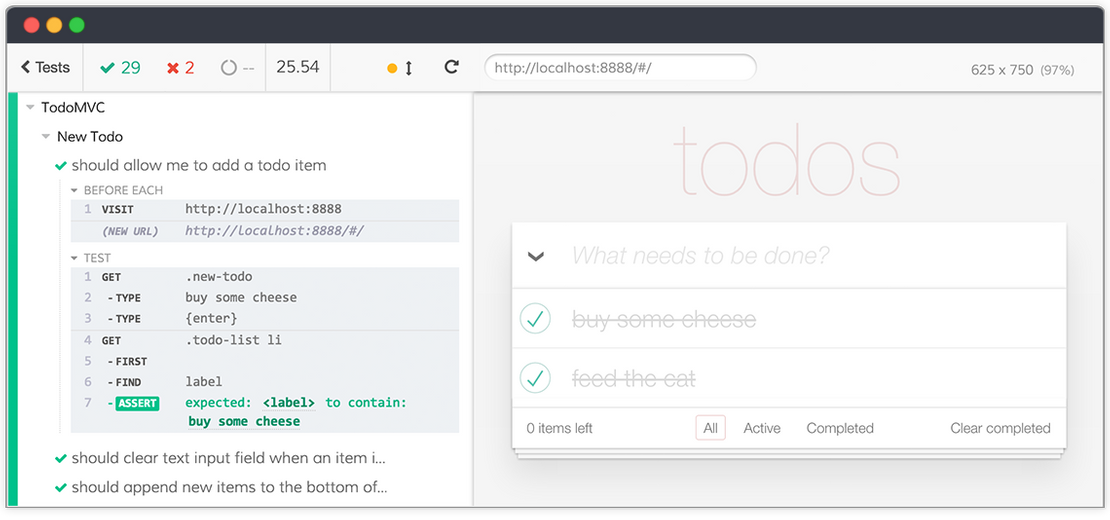
\includegraphics[width=1\textwidth]{images/cypress.png}
    \caption{Egy Cypress-ben futtatott E2E teszt}
    \label{fig:cypress-example}
\end{figure}

\subsection{Unit tesztelés}

A tesztelési piramis legalsó szintjén található a unit tesztelés. \textit{Unit test} alatt jellemzően egy olyan tesztet értünk, ami izolációban teszteli egy nagyon specifikus részét a kódnak. A pontos definíció ebben az esetben erősen vitatott, mert gyakorlatban a unit tesztelésnek több különböző stílusa létezik. Jellemzően ezek a stílusok eltérnek az izoláció mértékében, a tesztelt kód specificitásában és az ellenőrzések formájában is. Sok projekt továbbá kombinálja ezeket a különböző stílusokat az alkalmazás különböző rétegeiben.

\begin{figure}[H]
    \centering
    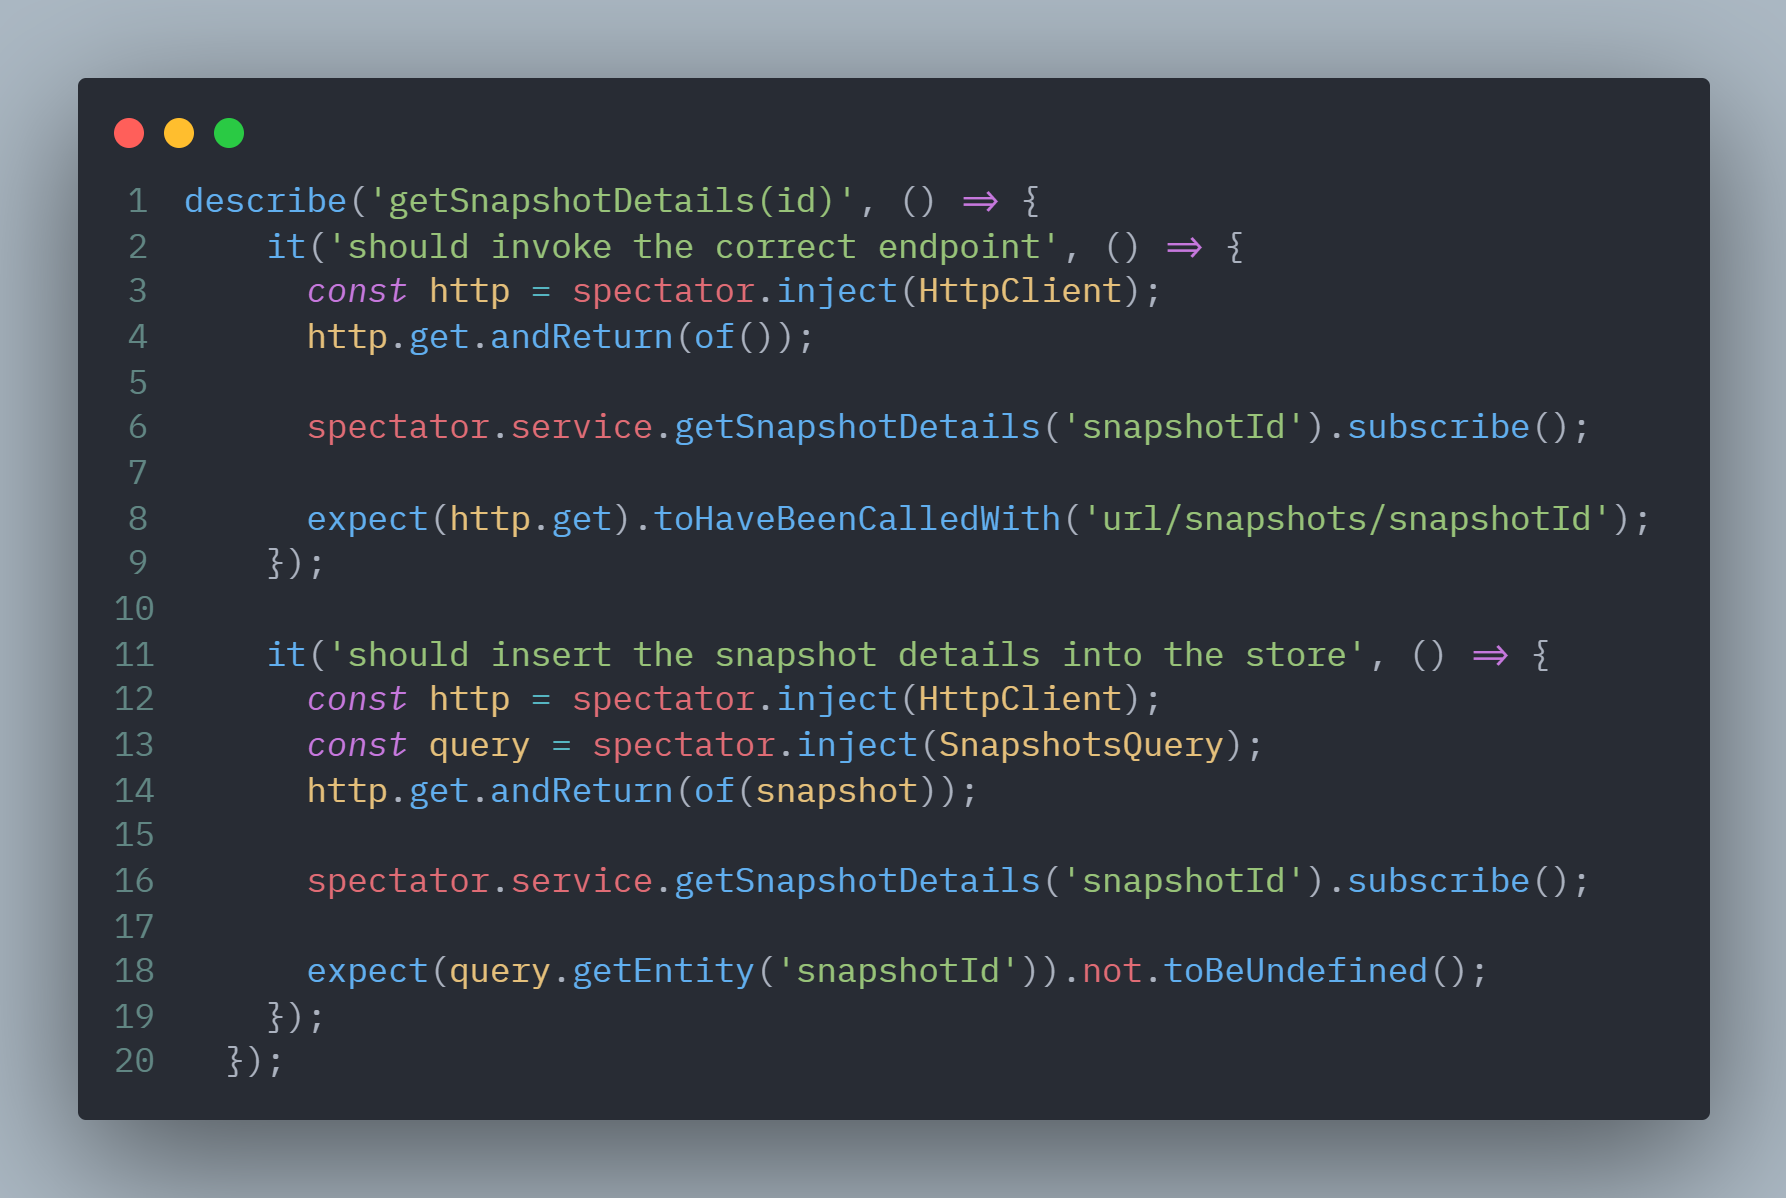
\includegraphics[width=0.8\textwidth]{images/unit-test.png}
    \caption{Unit teszt a Hestia UI projektből}
    \label{fig:unit-test-example}
\end{figure}

\begin{figure}[H]
    \centering
    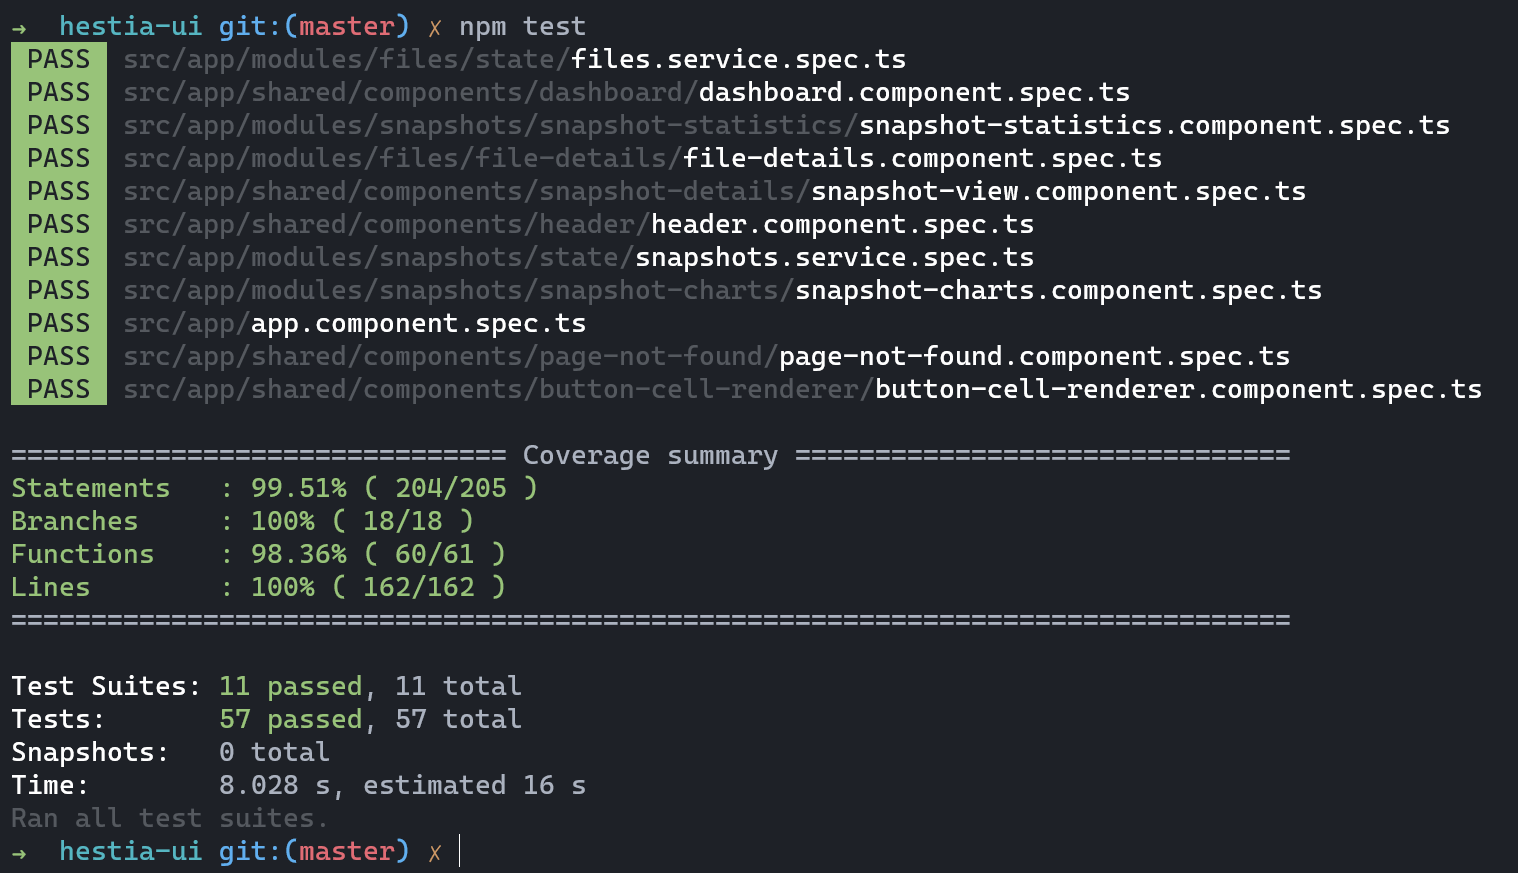
\includegraphics[width=0.8\textwidth]{images/testRun.png}
    \caption{Unit tesztek futtatása}
    \label{fig:unit-test-run-example}
\end{figure}

Definíciótól függetlenül azonban a unit tesztek célja világos: bizonyítsuk, hogy a kód, amit írtunk tényleg úgy viselkedik, ahogy szeretnénk. Tekinthetünk az ilyen tesztekre a szoftverfejlesztési világ kettős könyveléseként

\subsection{Teszt coverage}

Tisztáztuk a korábbiakban a tesztelés alapvető célját és a különböző szintjeit, azonban arról még nem esett szó, hogy milyen metrikákat tudunk kinyerni egy kódbázis tesztjeiből. Itt jön képbe a teszt coverage, ami azt mutatja, hogy a futattott tesztek milyen arányban hajtják meg az éles kódot, bizonyos szempontok szerint. Jellemzően a következő különböző szinten értelmezzük a coverage-et:
\begin{itemize}
    \item \textit{Statement coverage}: todo
    \item \textit{Line coverage}: todo
    \item \textit{Function coverage}: a kódbázisban lévő függvények
    \item \textit{Branch coverage}: vezérlési struktúrák ágainak coverage értéke
    \item \textit{Condition coverage}: boolean
\end{itemize}

\begin{figure}[H]
    \centering
    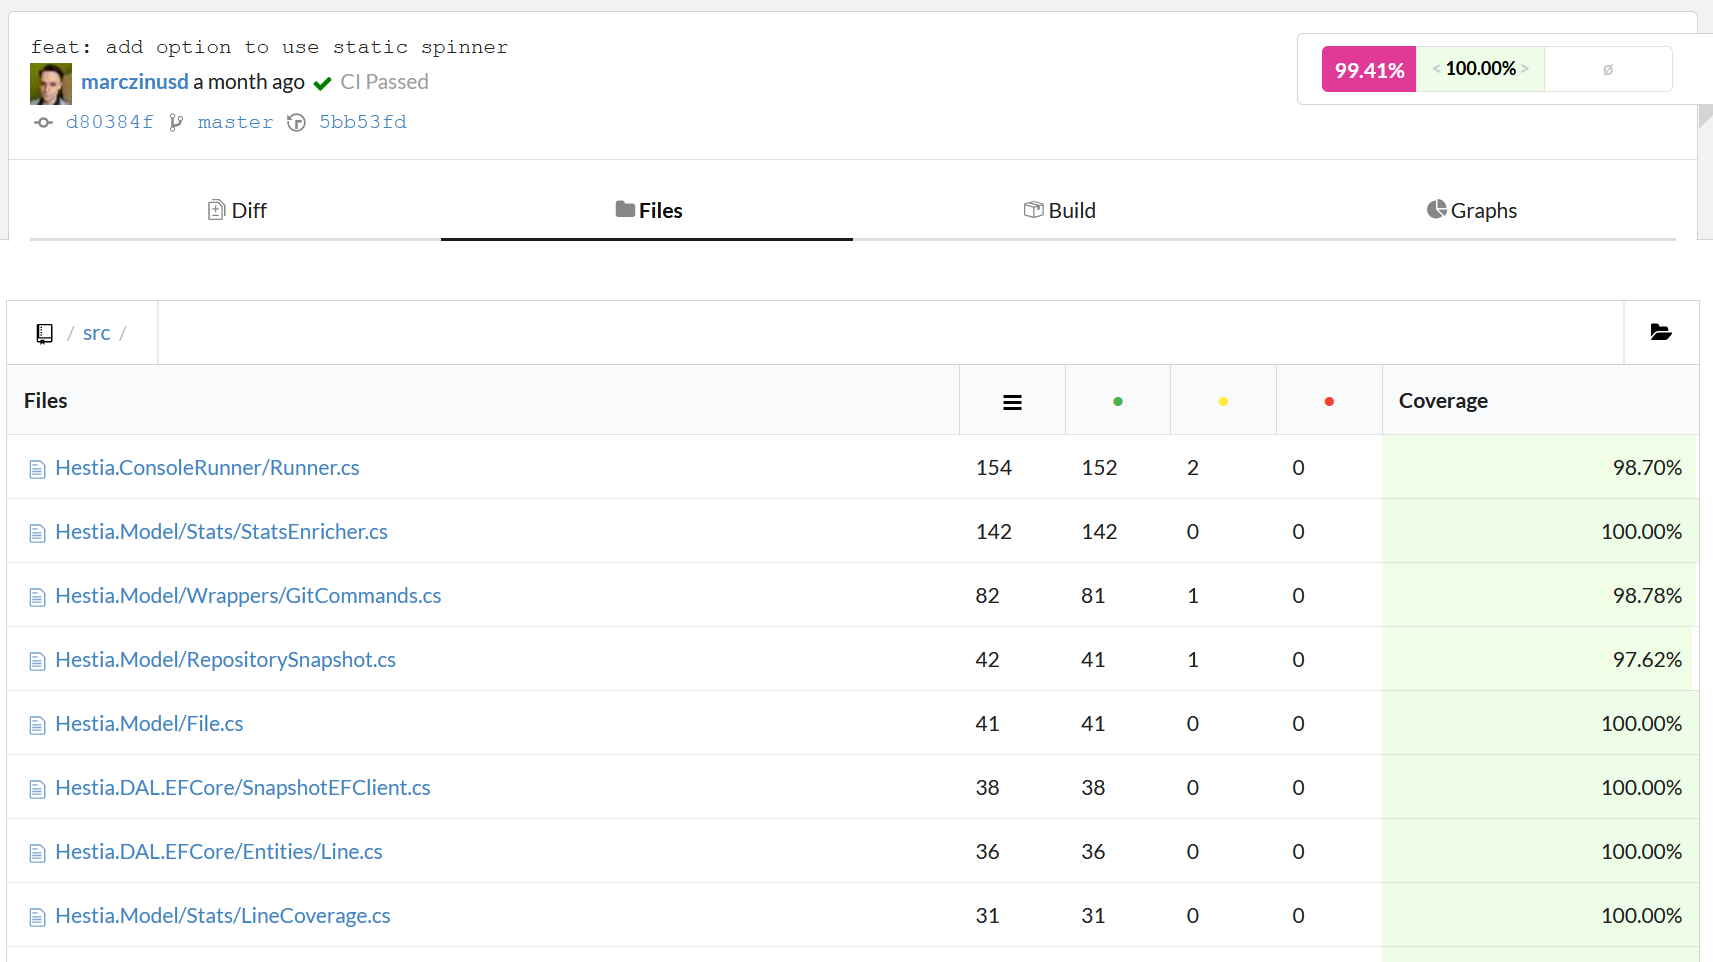
\includegraphics[width=1\textwidth]{images/codecov-report.png}
    \caption{Egy coverage report a codecov.io oldalról}
    \label{fig:codecov-example}
\end{figure}

Technikailag a tesztelési piramis minden szintjéből képezhető egy coverage report, de ahogy haladunk felfelé a hierarchiában, ez egyre nehezebb és kevésbé releváns lesz.

\section{A teszt coverage és git statisztikák közös vizsgálata}

Most, hogy körbejártuk két empirikus módját a kódminőség felmérésének, itt az ideje definiálni a kérdéseket, amiket ez a dipomamunka hivatott megvizsgálni.

Milyen relációban van a histórikus code coverage és a korábban definiált git statisztika? Hogyan viselkednek ezek az értékek "jó" és "rossz" minőségű kódbázisokon? Segít-e a megfelelő tesztelés abban, hogy a code smell-eket kordában tudjuk tartani?

